\documentclass{article}\usepackage[]{graphicx}\usepackage[]{color}
%% maxwidth is the original width if it is less than linewidth
%% otherwise use linewidth (to make sure the graphics do not exceed the margin)
\makeatletter
\def\maxwidth{ %
  \ifdim\Gin@nat@width>\linewidth
    \linewidth
  \else
    \Gin@nat@width
  \fi
}
\makeatother

\definecolor{fgcolor}{rgb}{0.345, 0.345, 0.345}
\newcommand{\hlnum}[1]{\textcolor[rgb]{0.686,0.059,0.569}{#1}}%
\newcommand{\hlstr}[1]{\textcolor[rgb]{0.192,0.494,0.8}{#1}}%
\newcommand{\hlcom}[1]{\textcolor[rgb]{0.678,0.584,0.686}{\textit{#1}}}%
\newcommand{\hlopt}[1]{\textcolor[rgb]{0,0,0}{#1}}%
\newcommand{\hlstd}[1]{\textcolor[rgb]{0.345,0.345,0.345}{#1}}%
\newcommand{\hlkwa}[1]{\textcolor[rgb]{0.161,0.373,0.58}{\textbf{#1}}}%
\newcommand{\hlkwb}[1]{\textcolor[rgb]{0.69,0.353,0.396}{#1}}%
\newcommand{\hlkwc}[1]{\textcolor[rgb]{0.333,0.667,0.333}{#1}}%
\newcommand{\hlkwd}[1]{\textcolor[rgb]{0.737,0.353,0.396}{\textbf{#1}}}%
\let\hlipl\hlkwb

\usepackage{framed}
\makeatletter
\newenvironment{kframe}{%
 \def\at@end@of@kframe{}%
 \ifinner\ifhmode%
  \def\at@end@of@kframe{\end{minipage}}%
  \begin{minipage}{\columnwidth}%
 \fi\fi%
 \def\FrameCommand##1{\hskip\@totalleftmargin \hskip-\fboxsep
 \colorbox{shadecolor}{##1}\hskip-\fboxsep
     % There is no \\@totalrightmargin, so:
     \hskip-\linewidth \hskip-\@totalleftmargin \hskip\columnwidth}%
 \MakeFramed {\advance\hsize-\width
   \@totalleftmargin\z@ \linewidth\hsize
   \@setminipage}}%
 {\par\unskip\endMakeFramed%
 \at@end@of@kframe}
\makeatother

\definecolor{shadecolor}{rgb}{.97, .97, .97}
\definecolor{messagecolor}{rgb}{0, 0, 0}
\definecolor{warningcolor}{rgb}{1, 0, 1}
\definecolor{errorcolor}{rgb}{1, 0, 0}
\newenvironment{knitrout}{}{} % an empty environment to be redefined in TeX

\usepackage{alltt}

\title{Problem Set 2}
\author{Kaylee, Carrie, Kritphong, Filipe and Klint \\ EDUC 252L}
\IfFileExists{upquote.sty}{\usepackage{upquote}}{}
\begin{document}
\maketitle
\section{Breaking the Classical Test Theory Model}

  \subsection{Coin Flips}
    Coin flips should not be reliable data - they're random!  To look at this a little more analytically:
    
      \[ \alpha = \frac{K}{K-1}\Bigg(1-\frac{\sum_{i=1}^{K}p_i(1-p_i)}{\sigma_{X}^{2}}\Bigg)\]
    
    The interesting thing to note here is that the probability of flipping heads is:
      \[p_i = 0.5 \]
    And the variance on the sum of $K$ coin flips will be:
      \[ \sigma_X = 0.25K \]
    Substituting in the formula for Cronbach's Alpha:
      \[ \alpha = \frac{K}{K-1}\Bigg(1-\frac{\sum_{i=1}^{K}(0.5)(1-0.5)}{0.25K}\Bigg)\]
    Cleaning up:
      \[ \alpha = \frac{K}{K-1}\Bigg(1-\frac{0.25K}{0.25K}\Bigg)\]
      \[ \alpha = \frac{K}{K-1}(1-1)\]
      \[ \alpha = 0 \]
    The expectation, then, is that $\alpha$ shoudl be zero for each situation.


\begin{knitrout}
\definecolor{shadecolor}{rgb}{0.969, 0.969, 0.969}\color{fgcolor}
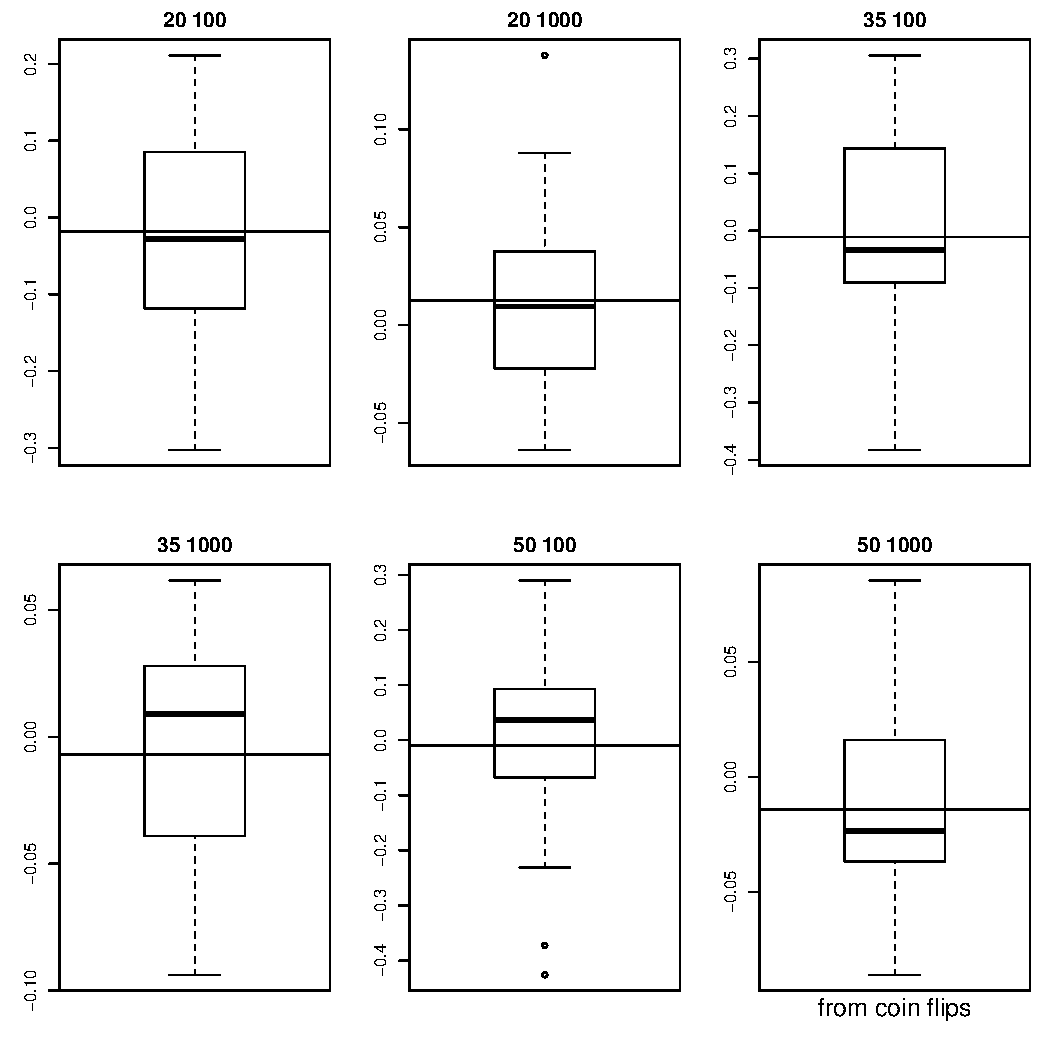
\includegraphics[width=\maxwidth]{figure/unnamed-chunk-1-1} 

\end{knitrout}

    These $\alpha$ plots make sense - they are centered around zero, as predicted, and as the number of items increases, $\alpha$ is more tightly clustered around zero.

  \subsection{Simulating Item Response Data}

\begin{knitrout}
\definecolor{shadecolor}{rgb}{0.969, 0.969, 0.969}\color{fgcolor}
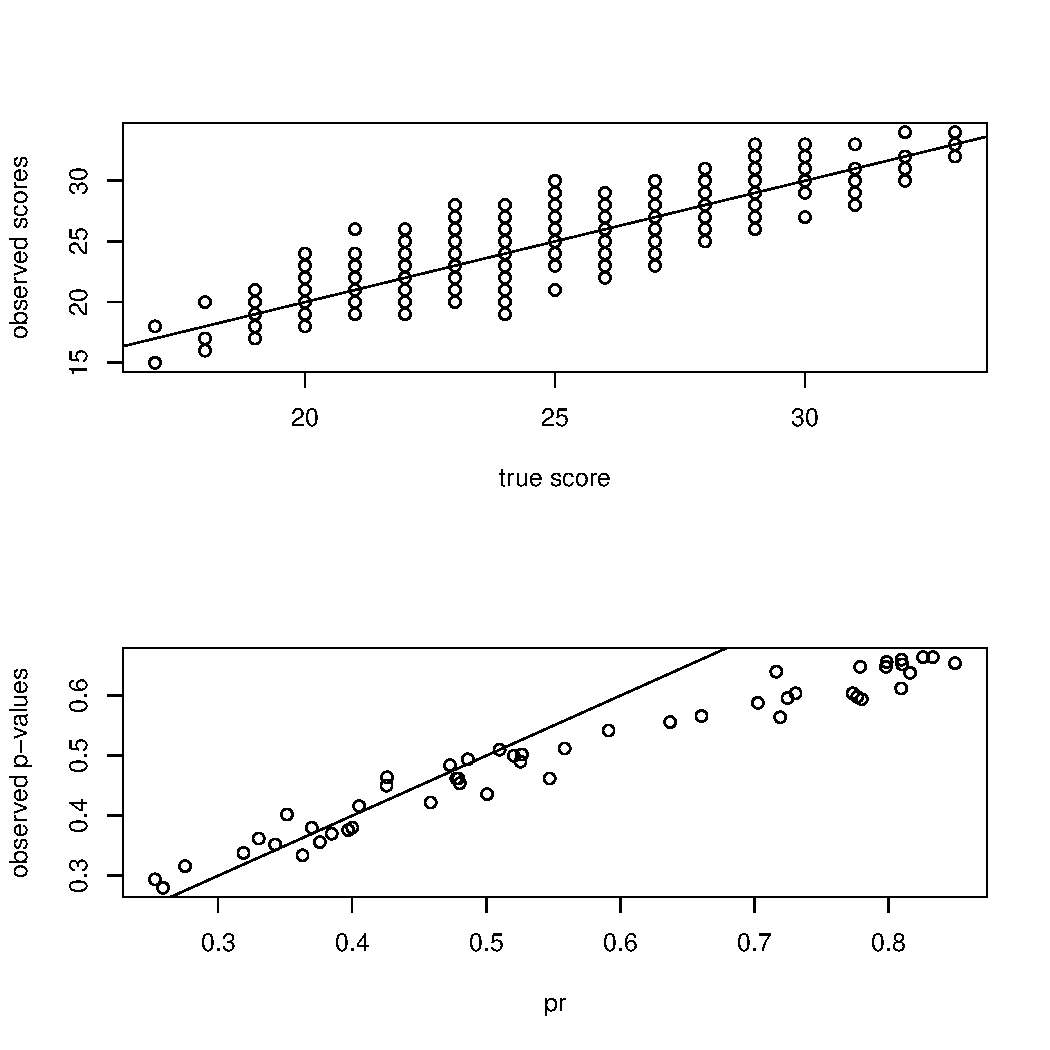
\includegraphics[width=\maxwidth]{figure/unnamed-chunk-2-1} 

\end{knitrout}

The feature of the data generation mechanism that makes the $\alpha$ values super low is that items are getting marked correctly (essentially) at random!  Even though the item responses generated correct p-values and test-level correlations, the data generation disregarded any internal structure you would expect.  More clearly stated, respondents of similar ability levels did not have similar item response profiles.

\begin{knitrout}
\definecolor{shadecolor}{rgb}{0.969, 0.969, 0.969}\color{fgcolor}
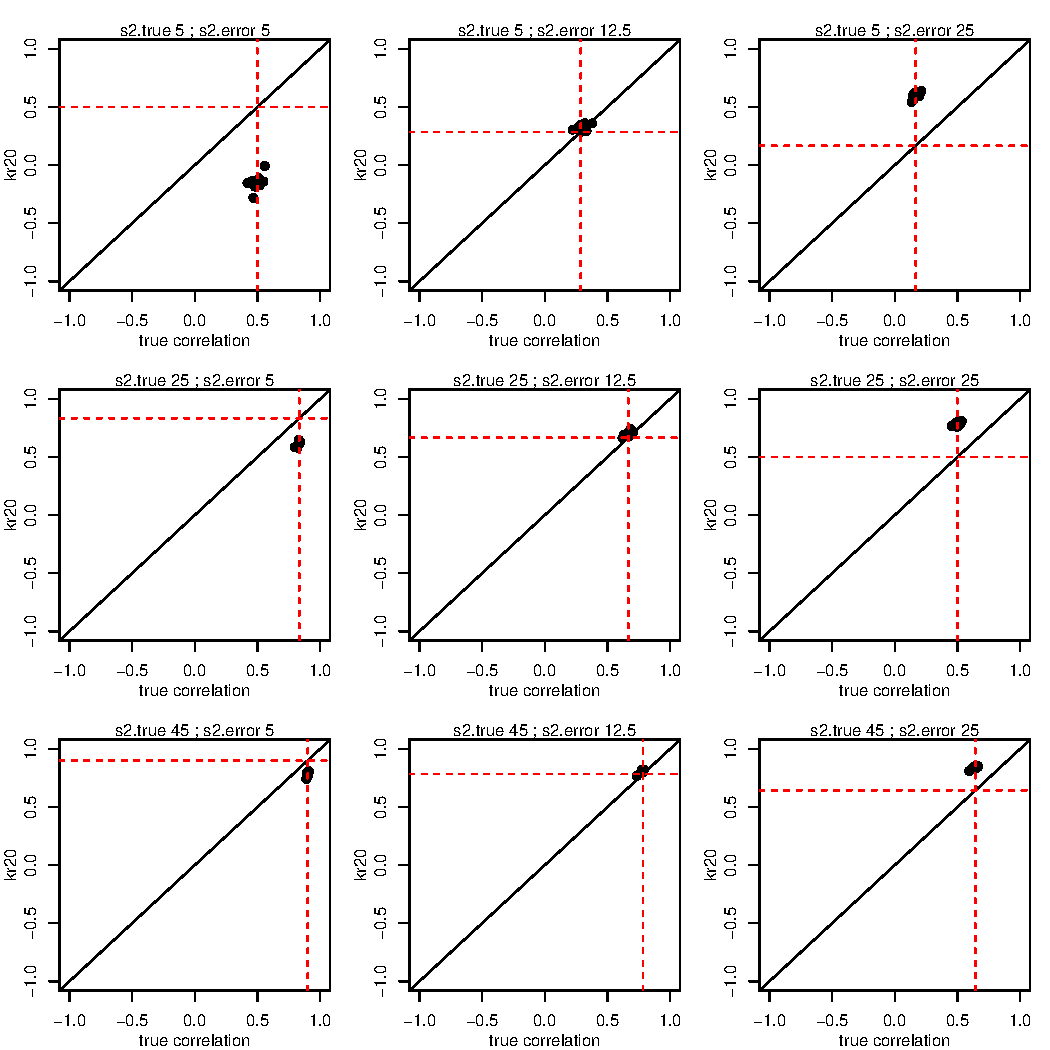
\includegraphics[width=\maxwidth]{figure/unnamed-chunk-3-1} 

\end{knitrout}

Looking at the resulting plots, it's clear that even with nonsensical item response data, the KR-20 estimate of reliability increases as a function of both true score variance and error variance.  This \em feels \em very wrong.  Increasing true score variance can be done by applying an instrument to a population it may not have been originally designed for.  Increasing error variance can be done by adding more items or manipulating the quality of items.  The challenge with feeling good about the CTT model is that KR-20 is both heavily valued and easily manipulated.  The worst part is that some of the behaviors that would increase a KR-20 value could have negative impacts on the validity of the instrument.

\pagebreak
\section{Different Link Functions}
\subsection{The Default}
\begin{knitrout}
\definecolor{shadecolor}{rgb}{0.969, 0.969, 0.969}\color{fgcolor}\begin{kframe}


{\ttfamily\noindent\itshape\color{messagecolor}{\#\# Loading required package: stats4}}

{\ttfamily\noindent\itshape\color{messagecolor}{\#\# Loading required package: lattice}}\end{kframe}
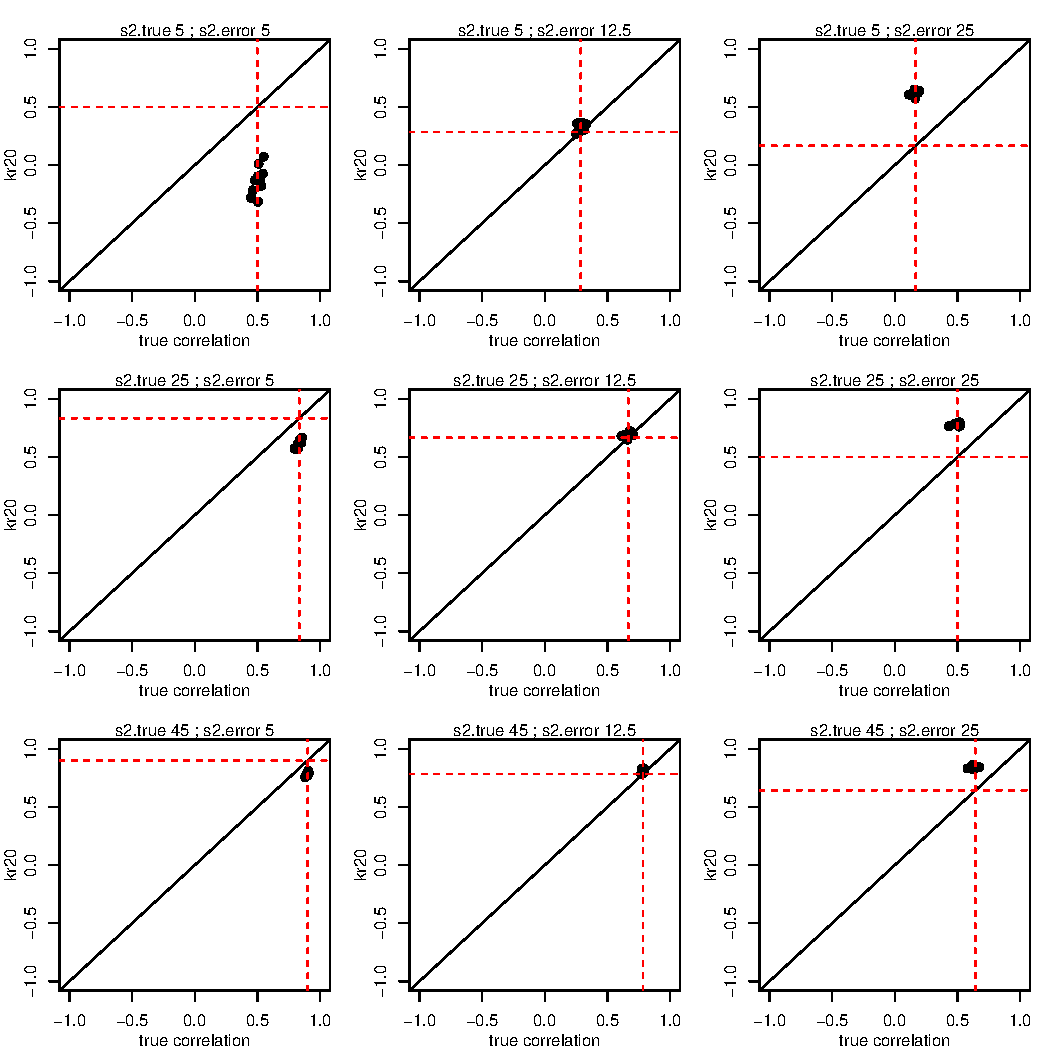
\includegraphics[width=\maxwidth]{figure/unnamed-chunk-4-1} 

\end{knitrout}

\subsection{The Normal}

\begin{knitrout}
\definecolor{shadecolor}{rgb}{0.969, 0.969, 0.969}\color{fgcolor}
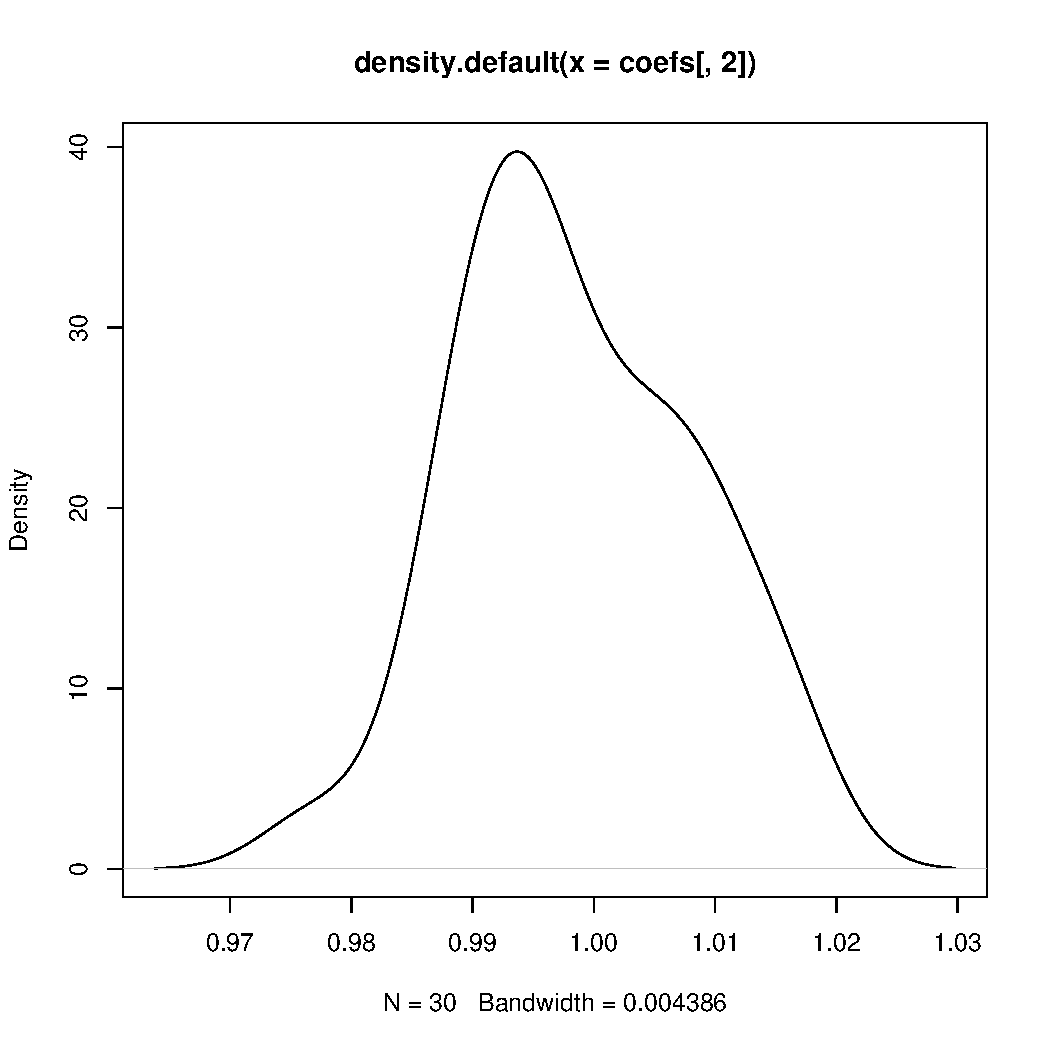
\includegraphics[width=\maxwidth]{figure/unnamed-chunk-5-1} 

\end{knitrout}

\subsection{Heavy Tails}

\begin{knitrout}
\definecolor{shadecolor}{rgb}{0.969, 0.969, 0.969}\color{fgcolor}
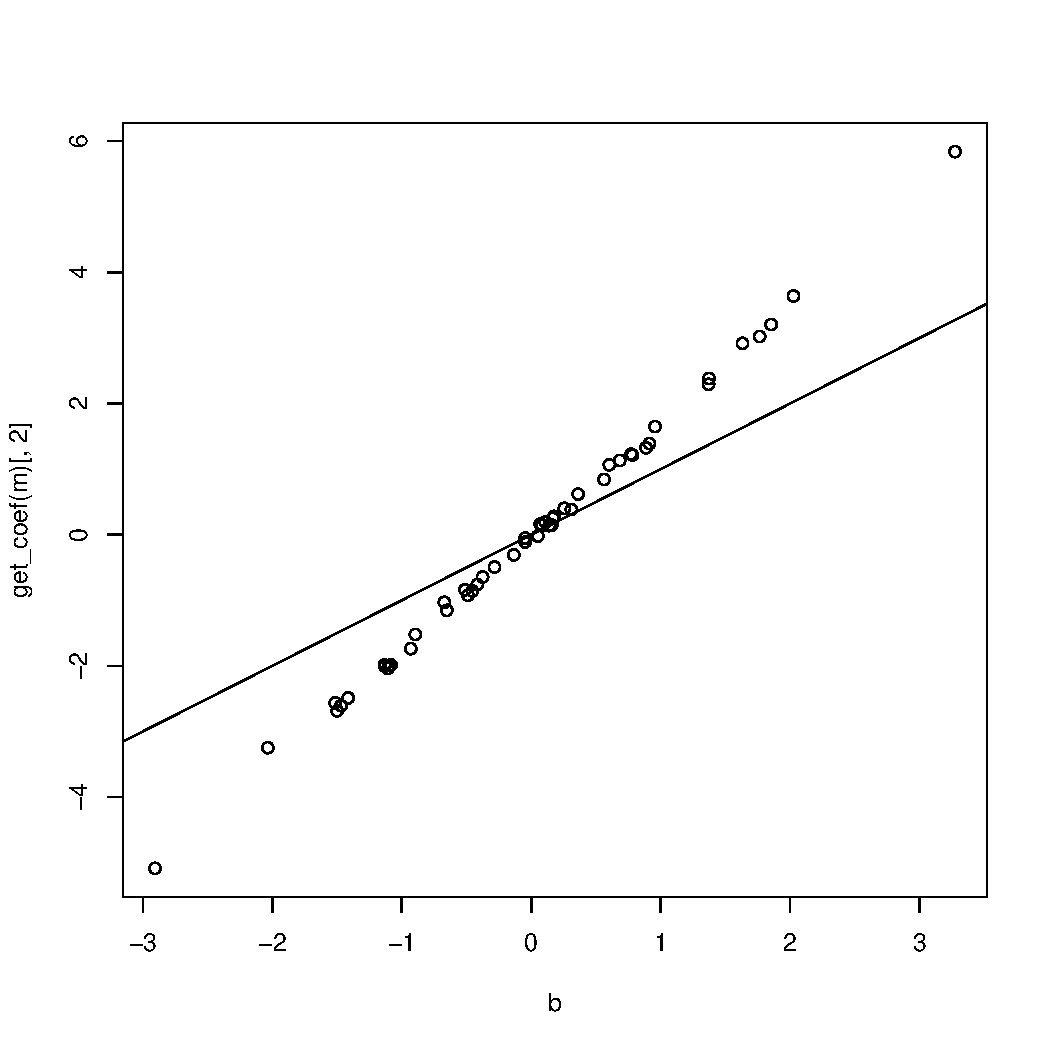
\includegraphics[width=\maxwidth]{figure/unnamed-chunk-6-1} 

\end{knitrout}

\subsection{Skewed}

\begin{knitrout}
\definecolor{shadecolor}{rgb}{0.969, 0.969, 0.969}\color{fgcolor}\begin{kframe}


{\ttfamily\noindent\itshape\color{messagecolor}{\#\# \\\#\# Attaching package: 'sn'}}

{\ttfamily\noindent\itshape\color{messagecolor}{\#\# The following object is masked from 'package:stats':\\\#\# \\\#\#\ \ \ \  sd}}\end{kframe}
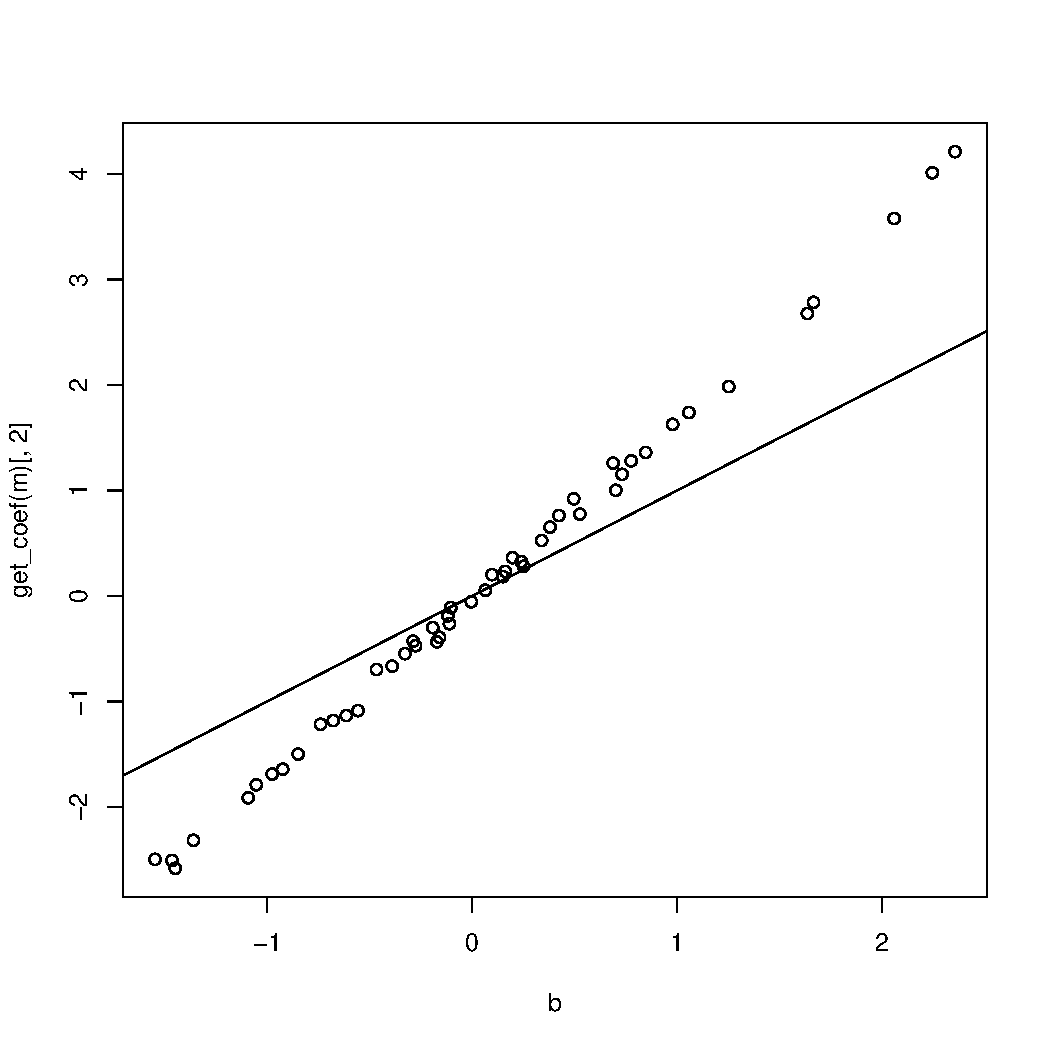
\includegraphics[width=\maxwidth]{figure/unnamed-chunk-7-1} 

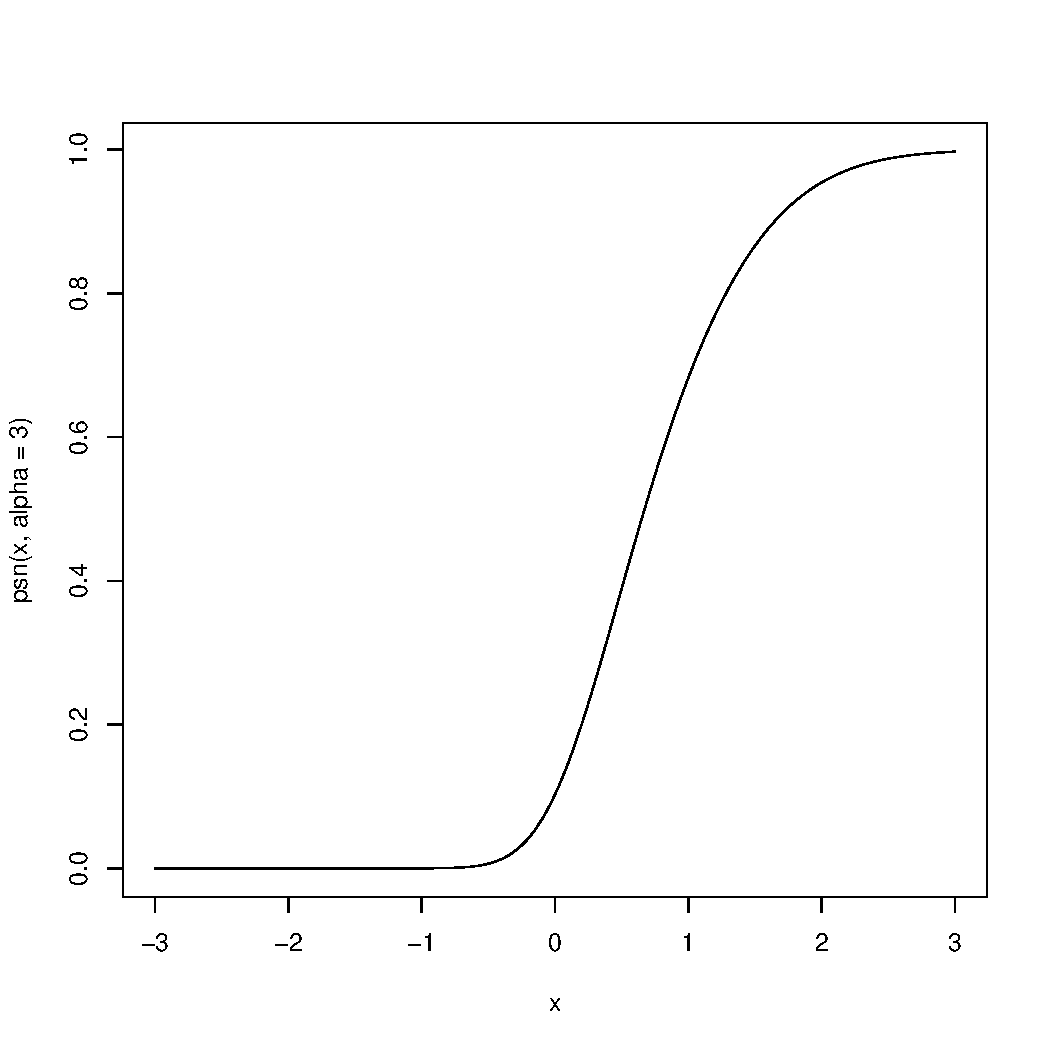
\includegraphics[width=\maxwidth]{figure/unnamed-chunk-7-2} 

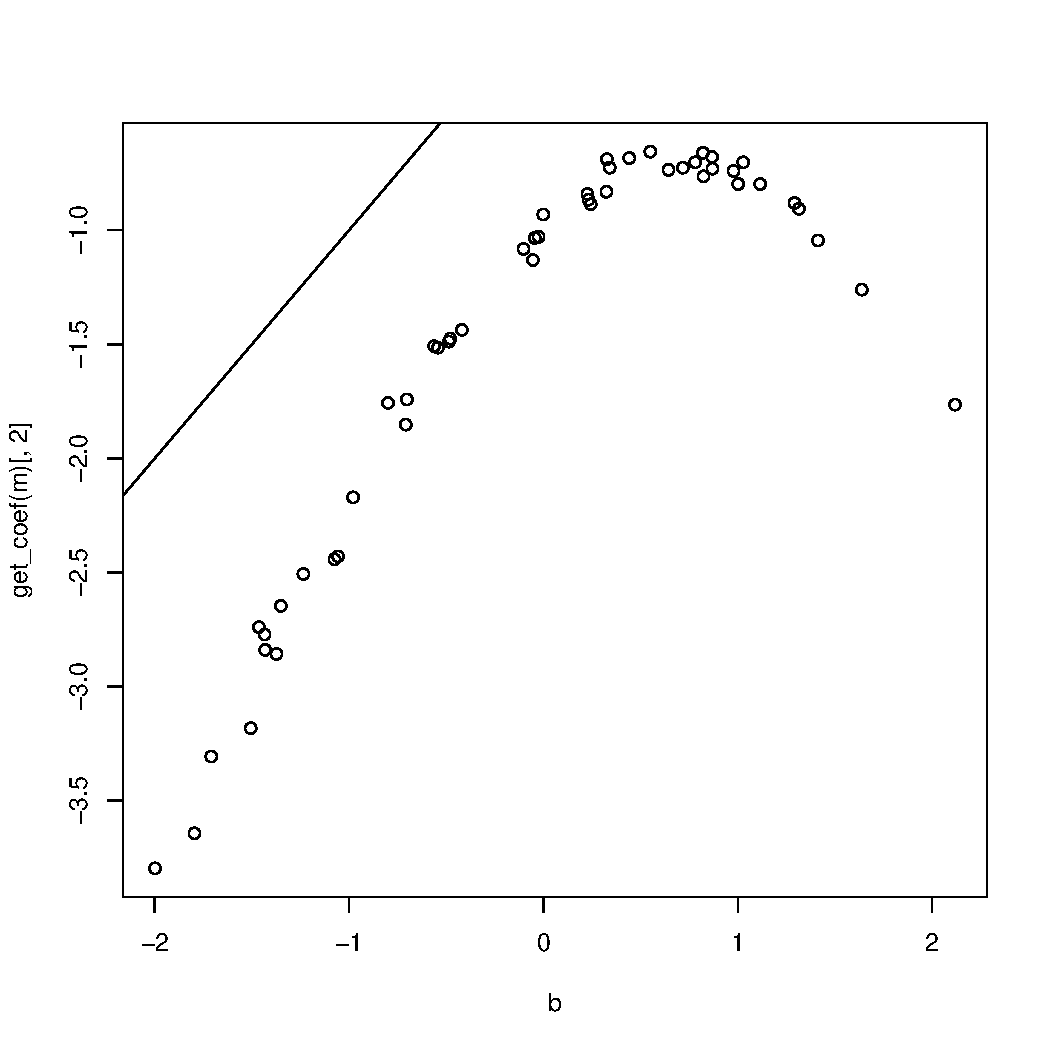
\includegraphics[width=\maxwidth]{figure/unnamed-chunk-7-3} 

\end{knitrout}


\end{document}
